% This LaTeX was auto-generated from MATLAB code.
% To make changes, update the MATLAB code and export to LaTeX again.

\documentclass{article}

\usepackage[utf8]{inputenc}
\usepackage[T1]{fontenc}
\usepackage{lmodern}
\usepackage{graphicx}
\usepackage{color}
\usepackage{hyperref}
\usepackage{amsmath}
\usepackage{amsfonts}
\usepackage{epstopdf}
\usepackage[table]{xcolor}
\usepackage{matlab}

\sloppy
\epstopdfsetup{outdir=./}
\graphicspath{ {./uloha1_gebhart_hurdzan_images/} }

\begin{document}

\begin{par}
\begin{flushleft}
\textbackslash{}title\{TPŘRS\}
\end{flushleft}
\end{par}

\begin{par}
\begin{flushleft}
\textbackslash{}author\{jan.geb.jan \}
\end{flushleft}
\end{par}

\begin{par}
\begin{flushleft}
\textbackslash{}date\{March 2022\}
\end{flushleft}
\end{par}


\vspace{1em}
\begin{par}
\begin{flushleft}
\textbackslash{}maketitle
\end{flushleft}
\end{par}

\vspace{1em}

\matlabtitle{Úloha 1. FREKVENČNÍ FILTR}

\begin{par}
\begin{flushleft}
TPŘRS 2022
\end{flushleft}
\end{par}

\begin{par}
\begin{flushleft}
Skupina: 4 (\textbf{B1 HP})
\end{flushleft}
\end{par}

\begin{par}
\begin{flushleft}
Vypracoval: Jan Gebhart, Tomáš Hurdzan
\end{flushleft}
\end{par}

\begin{par}
\begin{flushleft}
Dne: 9.3.2022
\end{flushleft}
\end{par}

\matlabheadingtwo{1. Navrhněte co nejednoudušší přenosovou funkci frekvečního filtru typu horní propust dle prototypu Čebyšev I, která bude vyhovovat nýsledujícím mezím:}


\begin{matlaboutput}
Mimimální počet pólů je 2
\end{matlaboutput}

\begin{matlaboutput}
mag_tmp = 0.7079
\end{matlaboutput}
\begin{matlaboutput}
omega_tmp = 7.3418e+03
\end{matlaboutput}

\begin{matlaboutput}
F_cheb =
 
  s^2 + 1.286e-12 s + 1.889e-08
  -----------------------------
     s^2 + 6688 s + 7.614e07
 
Continuous-time transfer function.
\end{matlaboutput}
\begin{center}
\includegraphics[width=\maxwidth{56.196688409433015em}]{figure_0.eps}
\end{center}
\matlabheadingtwo{2. V rámci yadaného schématu určete hodnty obecných dvojpólů aktivní RC operační sítě}

\begin{par}
\begin{flushleft}
\includegraphics[width=\maxwidth{35.82538886101355em}]{image_0}
\end{flushleft}
\end{par}

\begin{matlaboutput}
Teoretická hodnota R1 = 1322.889531 [ohm]
\end{matlaboutput}
\begin{matlaboutput}
Teoretická hodnota R2 = 9007.422016 [ohm]
\end{matlaboutput}
\begin{matlaboutput}
Teoretická hodnota R3 = 0.000000 [ohm]
\end{matlaboutput}
\begin{matlaboutput}
Teoretická hodnota R4 = Inf [ohm]
\end{matlaboutput}
\begin{matlaboutput}
Teoretická hodnota C1 = 0.000000 [ohm]
\end{matlaboutput}
\begin{matlaboutput}
Teoretická hodnota C2 = 0.000000 [ohm]
\end{matlaboutput}
\matlabheadingtwo{3. Určete typy a hodnoty pasivních dvojpólů pasivního RC článku, stejného typu a mezní frekvecí jako u aktivní sítě}

\begin{matlaboutput}
Teoretická hodnota R0 = 4793.823587 [ohm]
\end{matlaboutput}
\matlabheadingtwo{4. Odvoďte a spočtěte frekvenční přenos navrženého obvodového řešení filtru (bez i s přídavným RC článkem). Porovnejte logaritmické frekvenční charakteristiky spočtených přenosů s frekvenčními charakteristikami navržených teoretických přenosů.}


\begin{par}
\begin{flushleft}
Teoretický přenos Chebyshevova filtru je:
\end{flushleft}
\end{par}

\begin{matlaboutput}
F_cheb_t =
 
               1.102e-15 s^2
  ---------------------------------------
  1.102e-15 s^2 + 7.372e-12 s + 8.392e-08
 
Continuous-time transfer function.
\end{matlaboutput}
\begin{par}
\begin{flushleft}
Skutečný přenos Chebyshevova filtru je:
\end{flushleft}
\end{par}

\begin{matlaboutput}
F_cheb_s =
 
               1.136e-15 s^2
  ---------------------------------------
  1.136e-15 s^2 + 7.662e-12 s + 8.851e-08
 
Continuous-time transfer function.
\end{matlaboutput}
\begin{center}
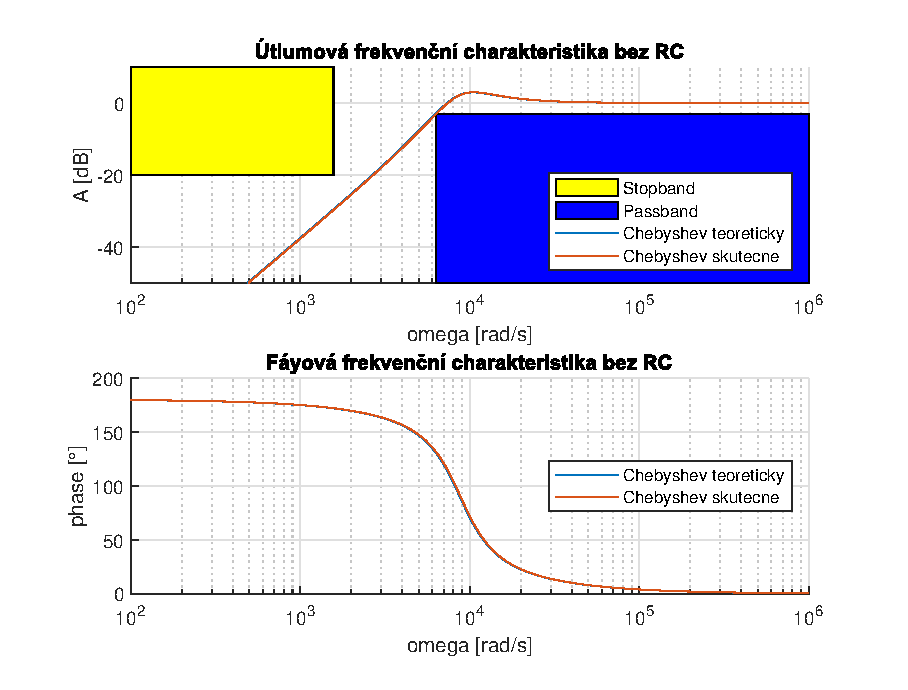
\includegraphics[width=\maxwidth{56.196688409433015em}]{figure_1.eps}
\end{center}

\begin{center}
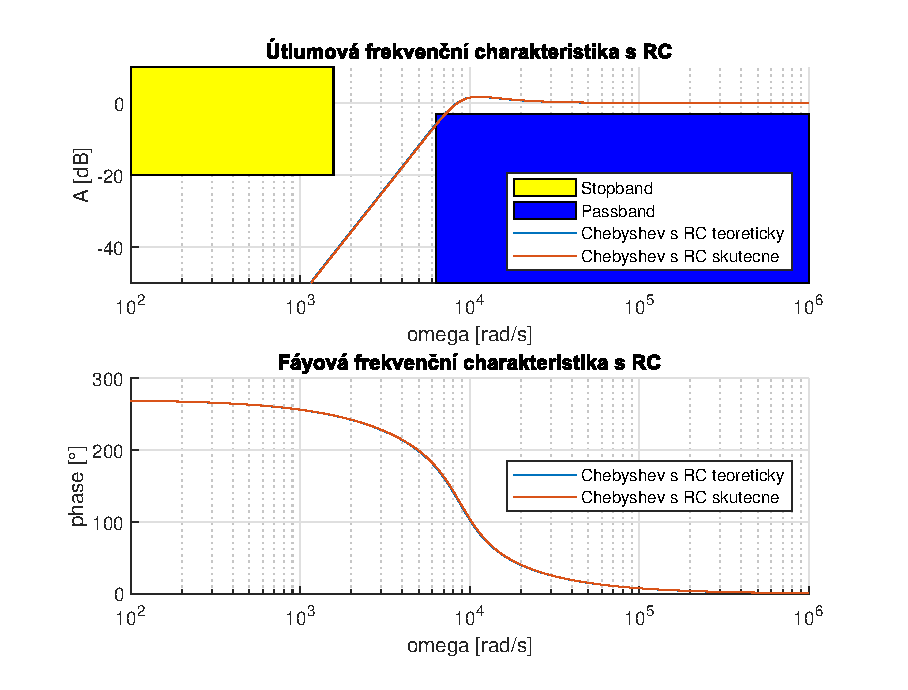
\includegraphics[width=\maxwidth{56.196688409433015em}]{figure_2.eps}
\end{center}
\matlabheadingtwo{5. Realizujte obvodová řešení na částečně univerzální desce plošných spojů. Potřebné hodnoty součástek sestavte sériově-paralelní kombinací standardizovaných hodnot R a C. Výsledné hodnoty ověřte měřením vybraných součástek.}

\begin{matlaboutput}
Chyba R0 = 1.454437 %
\end{matlaboutput}
\begin{matlaboutput}
Chyba R1 = 3.028780 %
\end{matlaboutput}
\begin{matlaboutput}
Chyba R2 = 2.368701 %
\end{matlaboutput}
\begin{matlaboutput}
Chyba C0 = 1.278620 %
\end{matlaboutput}
\begin{matlaboutput}
Chyba C1 = 2.266706 %
\end{matlaboutput}
\begin{matlaboutput}
Chyba C2 = 0.747384 %
\end{matlaboutput}

\matlabheading{6. Změřte logaritmickou amplitudovou frekvenční charakteristiku filtru (bez i s přídavným RC článkem) metodou postupného měření amplitudy procházejícího sinusového signálu s proměnnou frekvencí. Frekvence volte v rozsahu 50 Hz — 20 kHz v logaritmické řadě s preferencí okolí omega\_p. Porovnejte naměřené frekvenční charakteristiky obou variant s charakteristikami z předchozích bodů.}


\begin{center}
\includegraphics[width=\maxwidth{56.196688409433015em}]{figure_3.eps}
\end{center}

\begin{center}
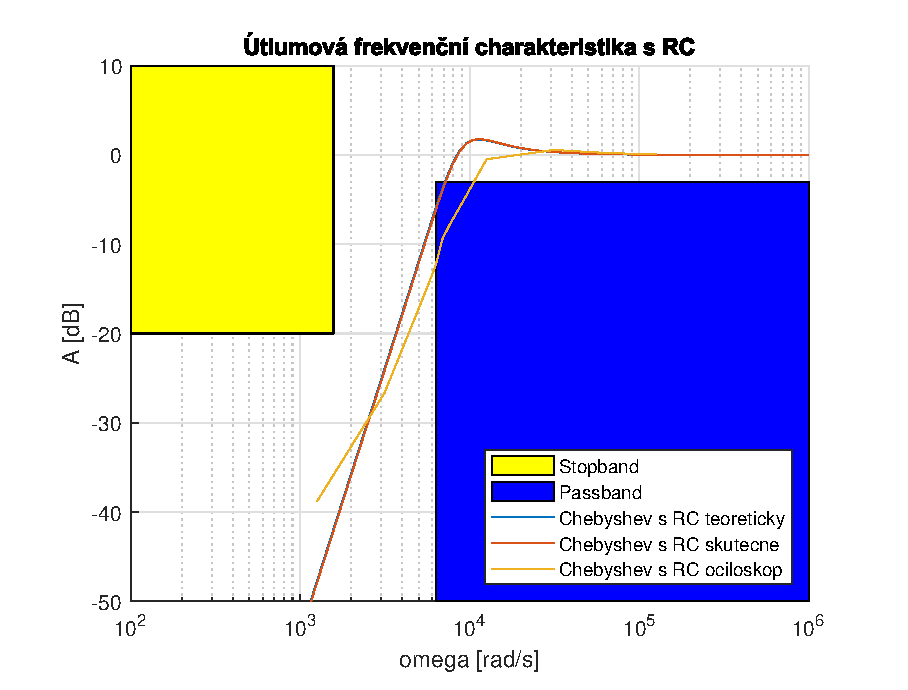
\includegraphics[width=\maxwidth{56.196688409433015em}]{figure_4.eps}
\end{center}

\matlabheadingtwo{7. Změřte fázové zpoždění na frekvenci 1kHz. Porovnejte naměřené hodnoty obou variant s fáyovými charakteristikami z bodu 4.}


\begin{center}
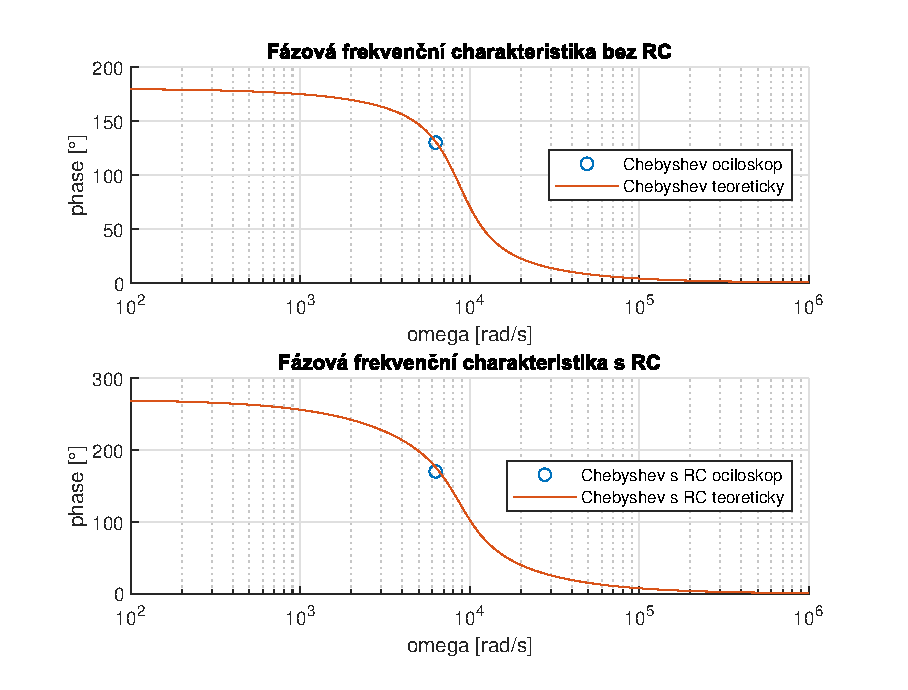
\includegraphics[width=\maxwidth{56.196688409433015em}]{figure_5.eps}
\end{center}
\matlabheadingtwo{8. Přeskočeno}

\matlabheadingtwo{9. Změřte logaritmickou amplitudovou frekvenční charakteristiku filtru (bez is přídavným RC článkem) metodou poměru amplitudových spekter výstupního signálu a vstupního signálu typu bílý šum. Porovnejte naměřené frekvenčni charakteristiky obou variant s charakteristikami přenosů z předchozích bodů.}



\begin{center}
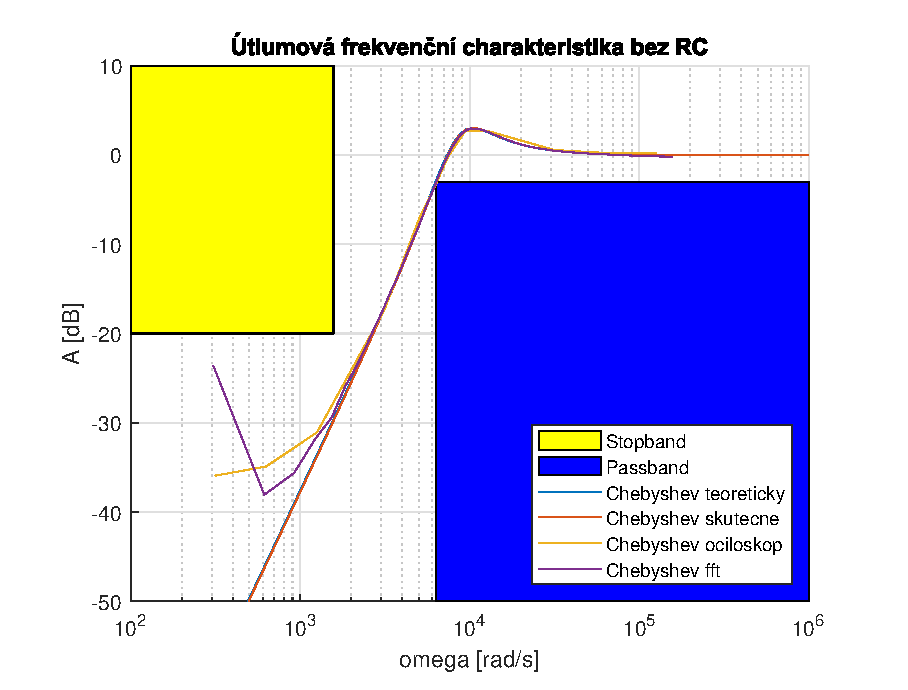
\includegraphics[width=\maxwidth{56.196688409433015em}]{figure_6.eps}
\end{center}

\begin{center}
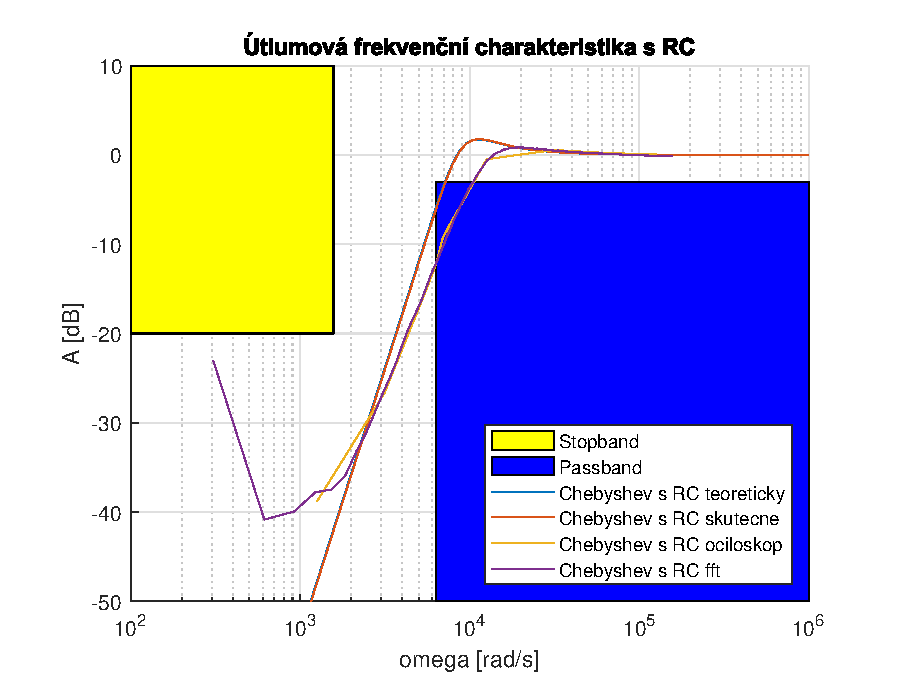
\includegraphics[width=\maxwidth{56.196688409433015em}]{figure_7.eps}
\end{center}
\matlabheadingtwo{10. Změřte přechodovou ftrekvenční charakteristiku filtru (bez i s přídavným RC článkem) metodou vybuzení filtru napětovým skokem 0 -1 V. Porovnejte neměřené charakteristiky obou variant s přechodovýmí charakteristikami spočtených přenosů.}



\begin{center}
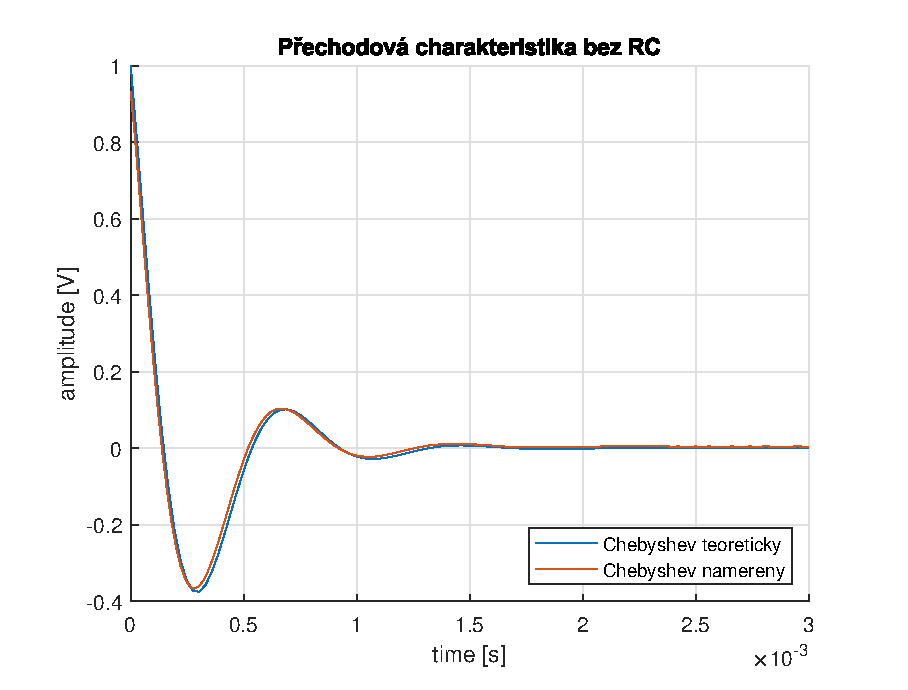
\includegraphics[width=\maxwidth{56.196688409433015em}]{figure_8.eps}
\end{center}

\begin{center}
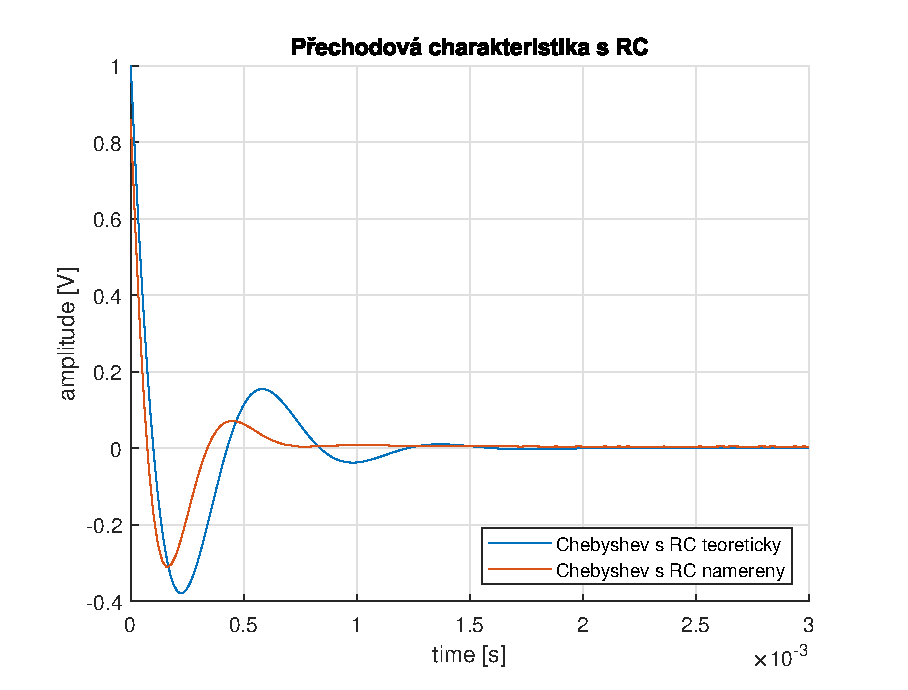
\includegraphics[width=\maxwidth{56.196688409433015em}]{figure_9.eps}
\end{center}
\matlabheadingtwo{11. Závěr}

\begin{par}
\begin{flushleft}
TODO
\end{flushleft}
\end{par}

\end{document}
